\documentclass{beamer} % Gliederung im Kopf, sections und subsections
\setbeamertemplate{navigation symbols}{}%remove navigation symbols

\usepackage{tikz}
\usetikzlibrary{shapes,arrows,positioning,chains,fit,calc,matrix,decorations.pathreplacing}
\usepackage{xcolor}
\usetikzlibrary{intersections}


\usepackage{tikz}
\usetikzlibrary{arrows,decorations.pathmorphing,backgrounds,positioning,fit,petri}
\renewcommand*{\familydefault}{\sfdefault}

\tikzset{forestyle/.style = {rectangle, thick, minimum width = 5cm, minimum height = 0.5cm, text width = 4.5cm, outer sep = 1mm},
  pre/.style={<-, shorten <=1pt, >=stealth, ultra thick},
  extend/.style={<-,dashed, shorten <=1pt, >=stealth, ultra thick}}



\def\firstcircle{[name path=firstcircle] (0,0) circle (3cm)}
\def\secondcircle{[name path=secondcircle] (55:3.11111cm) circle (3cm)} %No idea how the numbers selected work; they were derived from what I found online. They seem to function though!
\def\thirdcircle{[name path=thirdcircle] (0:3.5cm) circle (3cm)}


\mode<presentation>

\begin{document}

\begin{frame}\begin{center}
	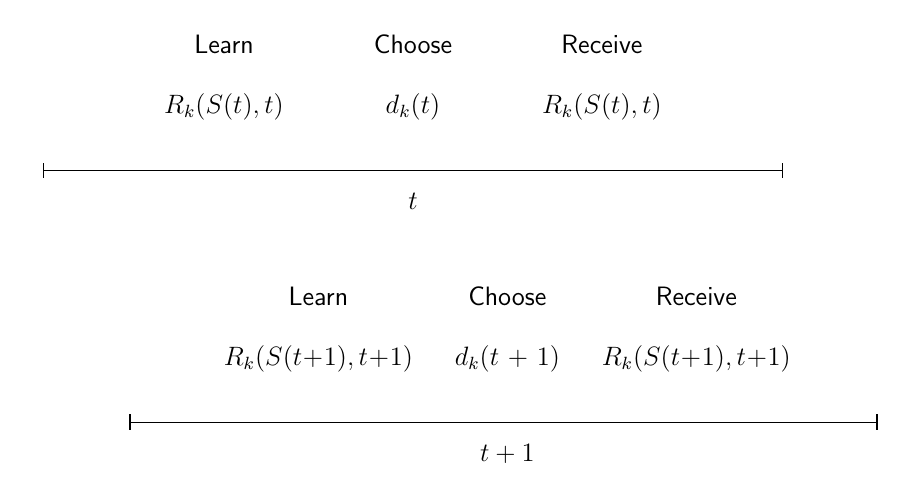
\begin{tikzpicture}[scale=1.0, every node/.style={scale=0.8}]

	\tikzset{
	eqblock/.style={text width=3cm,align=center}
	}

	% Nodes
	\node (left) {};
	\node[below right=3cm and 1cm of left] (bottom_left) {};
	\node[node distance=12cm, right of=left] (right) {};
	\node[node distance=12cm, right of=bottom_left] (bottom_right) {};

	\node[node distance=6cm, right of=left, yshift=-.5cm] (t1) {\large$t$};
	\node[node distance=6cm, right of=bottom_left, yshift=-.5cm] (t2) {\large$t+1$};

	\node[eqblock, above of=left, xshift=3cm] (eq1) {\large$R_k(S(t),t)$};
	\node[eqblock, above of=left, xshift=6cm] (eq2) {\large$d_k(t)$};
	\node[eqblock, above of=left, xshift=9cm] (eq3) {\large$R_k(S(t),t)$};
	\node[eqblock, above of=bottom_left, xshift=3cm] (eq4) {\large$R_k(S(t+1),t+1)$};
	\node[eqblock, above of=bottom_left, xshift=6cm] (eq6) {\large$d_k(t+1)$};
	\node[eqblock, above of=bottom_left, xshift=9cm] (eq5) {\large$R_k(S(t+1),t+1)$};

	\node[above of=eq1, node distance=1cm] (text2) {\large Learn};
	\node[above of=eq2, node distance=1cm] (text3) {\large Choose};
	\node[above of=eq3, node distance=1cm] (text1) {\large Receive};
	\node[above of=eq4, node distance=1cm] (text4) {\large Learn};
	\node[above of=eq6, node distance=1cm] (text5) {\large Choose};
	\node[above of=eq5, node distance=1cm] (text6) {\large Receive};

	% Lines
	\draw[|-|] (left) -- (right);
	\draw[|-|] (bottom_left.center) -- (bottom_right);

	\end{tikzpicture}\end{center}\end{frame}


\end{document}
